
\begin{frame}{Annexe}{Morphing Rectangle}

\begin{figure}[H]
\centerline{
   \subfigure[]{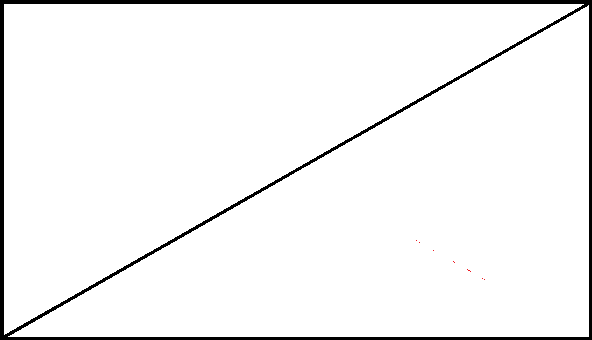
\includegraphics[scale=0.25]{img/morph-rectangle5.png}}
   \subfigure[]{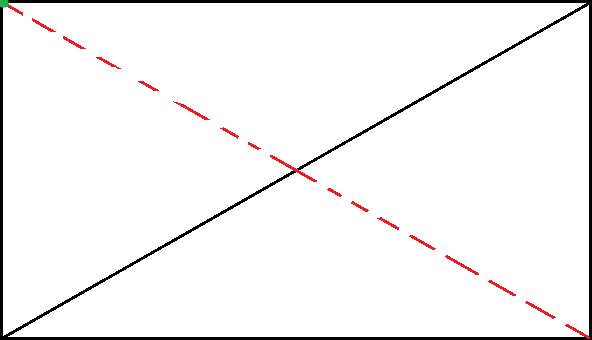
\includegraphics[scale=0.25]{img/morph-rectangle4.png}}
   \subfigure[]{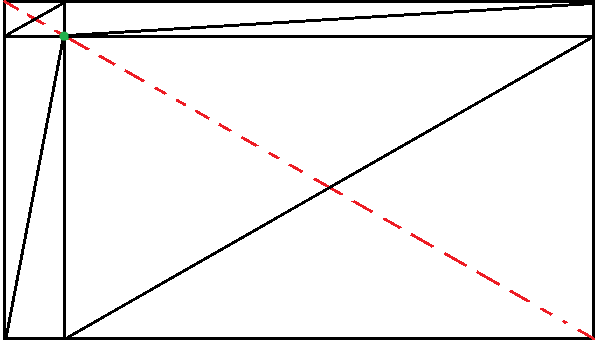
\includegraphics[scale=0.25]{img/morph-rectangle3.png}}
   }
\end{figure}
\begin{figure}[H]
   \subfigure[]{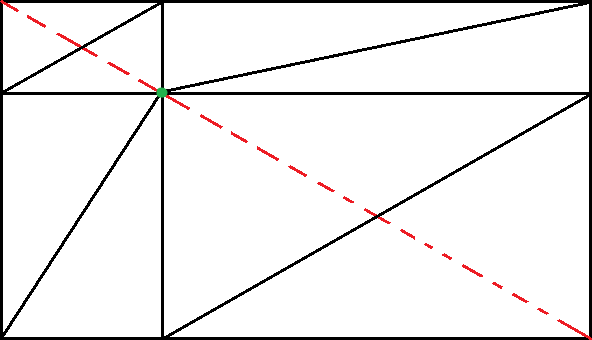
\includegraphics[scale=0.25]{img/morph-rectangle2.png}}
   \subfigure[]{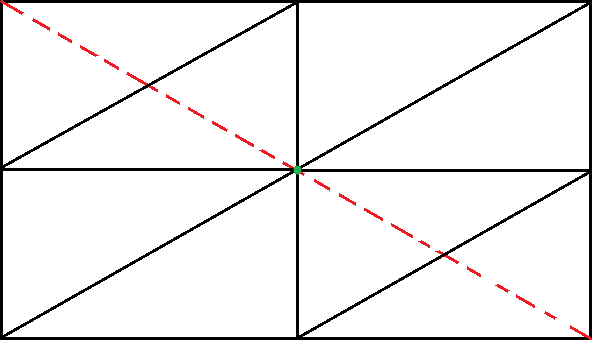
\includegraphics[scale=0.25]{img/morph-rectangle1.png}}
   
   \caption{Augmentation du niveau de détail}
\end{figure}
    
\end{frame}

\begin{frame}{Morphing}{}
 Le morphing supprime les trous aux frontières entre zones de niveaux différents.Ce procédé s'applique indépendamment sur chacun des points. La direction du morph a été renseignée par Patch. Son intensité dépend de la distance est du niveau de détail actuel.
 \begin{figure}[!b]
\centerline{
   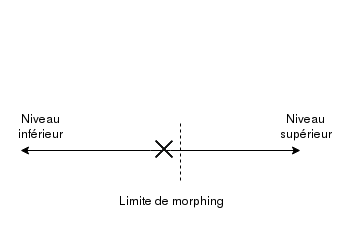
\includegraphics[scale=0.35]{img/morphing1.png}
   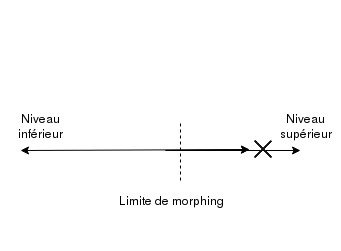
\includegraphics[scale=0.35]{img/morphing2.png}
   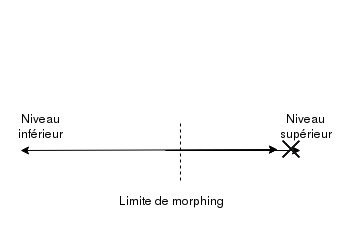
\includegraphics[scale=0.35]{img/morphing3.png}
   }
   \centerline{
   \subfigure[]{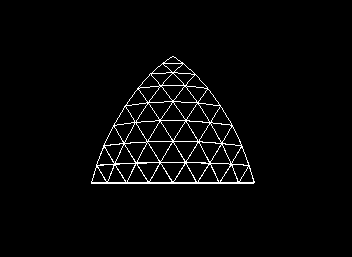
\includegraphics[scale=0.3]{img/morphingS1.png}}
   \subfigure[]{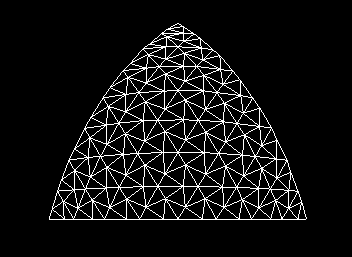
\includegraphics[scale=0.3]{img/morphingS2.png}}
   \subfigure[]{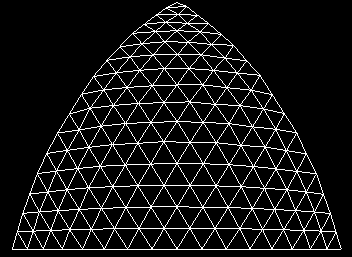
\includegraphics[scale=0.3]{img/morphingS3.png}}
   }
\end{figure}
 \end{frame}